\section{Marco Aplicativo}

\subsection{Método de Desarrollo}

Para lograr cumplir con los objetivos planteados en el Capítulo 2, es necesario definir un
esquema o metodología de trabajo que permita la elaboración de un conjunto de
lineamientos de manera estructurada y organizada. Por lo tanto, se hace uso de el método de 
Desarrollo Rápido de Aplicaciones (RAD), el cual permite la iteración rápida y continua
de pequeños objetivos para alcanzar la meta final.

RAD es un proceso de desarrollo de software que
integra un conjunto de técnicas, lineamientos y herramientas que permiten llevar a cabo, en
cortos periodos de tiempo, la implementación de funcionalidades en un sistema, de tal manera que
satisfacen las necesidades del cliente \cite{23}. Siguiendo esta metodología, el software
evoluciona y crece durante el proceso de desarrollo en base a la retro alimentación que
se tiene con el cliente. De esta manera, se realizan múltiples entregas de una tarea que
contiene las nuevas funcionalidades esperadas.

Por medio de RAD, fue posible la implementación de la solución al problema previamente planteado.
La misma está desarrollada como un servicio web API conformado por:

\begin{itemize}

\item Un modulo de extracción de revisiones de artículos wiki.

\item Un modulo de almacenamiento de datos distribuido por medio de MongoDB.

\item Un modulo de consulta de los artículos wiki extraídos y sus correspondientes revisiones.

\item Y, por último, un modulo de consulta de métricas generales de las revisiones extraídas, incluyendo: totalizaciones, promedios y moda.

\end{itemize}

La siguiente figura representa la vista general de la arquitectura de la aplicación, y como la misma interactuá con
las aplicaciones clientes que consumen el servicio.

\begin{figure}[H]
	\centering
		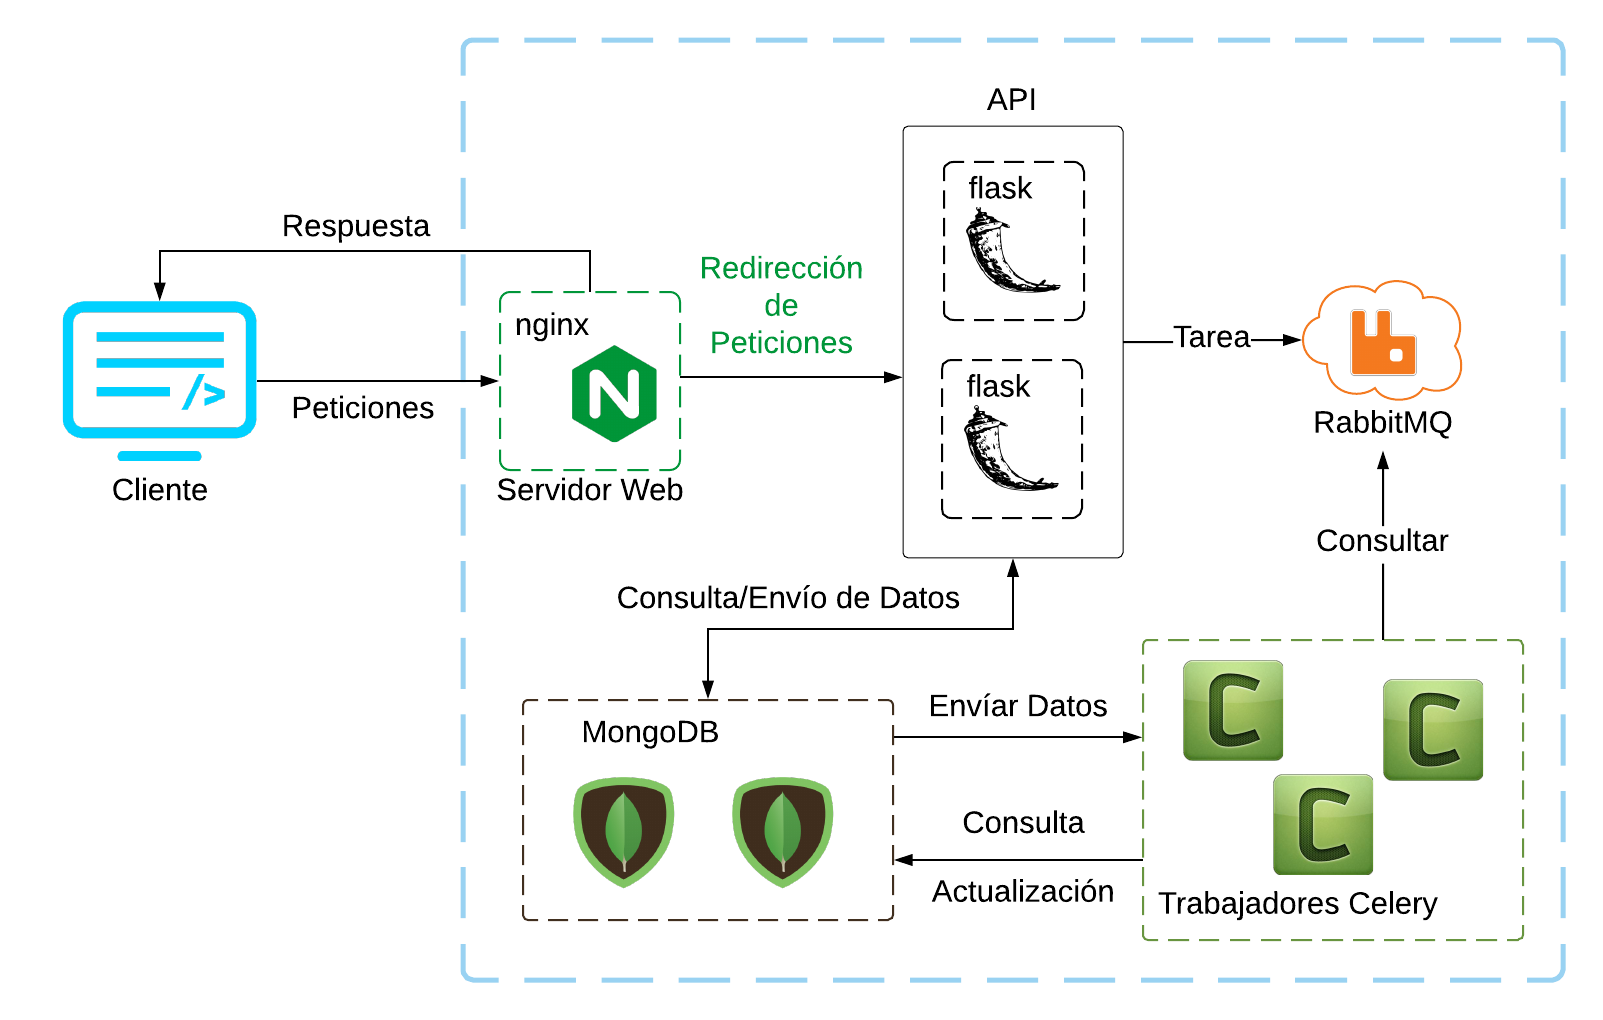
\includegraphics[width=.6\textwidth]{figures/diagram_general}
	\caption{Arquitectura general de la aplicación.}
	\label{fig:diagram_general}}

\end{figure}


\subsection{API}

El servicio web, diseñado para atender las solicitudes de extracción y consulta de las revisiones, hace uso del lenguaje de programación Python en su versión 2.7.10 y el uso del framework Flask v0.12. 
Ambas tecnologías permiten la asignación de rutas específicas para cada módulo
y la atención de peticiones.

La interacción entre el servicio y una aplicación cliente puede ser apreciada en la figura \ref{fig:diagram_api_1}.
Esta interacción se basa en la petición de un recurso o de un proceso, por parte de una aplicación cliente, a una ruta del servidor
web (endpoint). La petición puede incluir parámetros opcionales para: la paginación de resultados, filtros o cualquier
otro tipo de entrada que sea necesaria para procesar la solicitud; por ejemplo, el idioma del artículo a extraer.

\begin{figure}[H]
	\centering
		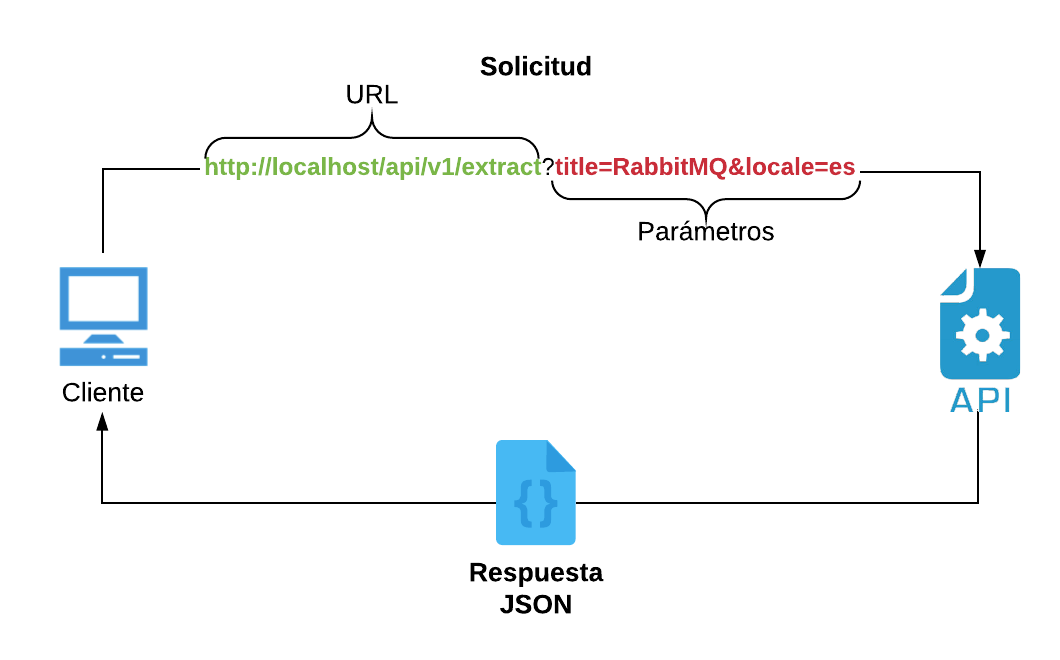
\includegraphics[width=1\textwidth]{figures/diagram_api_1}
	\caption{Interacción entre una aplicación cliente y el API.}
	\label{fig:diagram_api_1}
\end{figure}



Algunos de estos procesos como el de extracción de historiales son llevados a cabo por medio de Celery. Entre los componentes de la 
aplicación existen múltiples computadores denominados nodos que están conectados entre si por medio de RabbitMQ.
Cada nodo ejecuta un proceso de Celery llamado trabajador (worker), que constantemente esta en la búsqueda de tareas para su 
ejecución. Estas tareas son generadas desde la aplicación principal que recibe las peticiones de un cliente, en donde se 
genera un identificador único para cada una de ellas y se colocan en una cola de espera por medio de RabbitMQ. Cuando un nodo 
worker extrae una tarea de la cola de espera, el mismo la ejecuta en segundo plano y genera, de forma constante, mensajes que
indican el progreso de ejecución hasta su culminación.


El API consta de las siguientes rutas de acceso (endpoints):

\begin{itemize}
	\item /api/v1/articles
	\item /api/v1/revisions
	\item /api/v1/extract
	\item /api/v1/avg
	\item /api/v1/count
	\item /api/v1/mode
	\item /api/v1/status/<task_id>
\end{itemize}

* Nginx
* Flask

\subsubsection{Extracción de Historiales}

Para la extracción de historiales se hace uso de la ruta de acceso /api/v1/extract, la cual tiene como parámetros:
title, que se refiere al título del del artículo; url, representa la ruta completa de un artículo, por ejemplo: 
https://en.wikipedia.org/wiki/The_Lord_of_the_Rings; y por último, locale, el cual índica el idioma del artículo y 
es completamente opcional, puesto que el sistema asume el inglés como lenguaje por defecto o lo extrae del parámetro 
url. Es necesario proporcionar el parámetro url o title de forma obligatoria para poder llevar a cabo la extracción.

En la siguiente figura se puede apreciar dos ejemplos del uso de los parámetros url, title y locale.

\begin{figure}[H]
	\centering
		
\includegraphics[width=1\textwidth]{figures/extract_url_format}
	\caption{Parámetros para la extracción de historiales.}
	\label{fig:extract_url_format}
\end{figure}

Una vez recibida la petición, se genera el id de la tarea, se coloca en la cola de espera y se construye la respuesta a la petición
con un nuevo URL que contiene id anteriormente mencionado y el nombre del proceso, extrat_article. Este URL permite consultar el progreso del proceso de extracción y puede ser apreciado en la siguiente figura:

\begin{figure}[H]
	\centering
		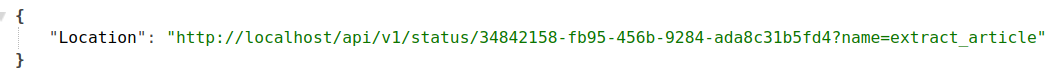
\includegraphics[width=1\textwidth]{figures/extract_response}
	\caption{Respuesta a una petición de extracción de historiales de un artículo.}
	\label{fig:extract_response}
\end{figure}

 y se ubica en una cola de espera hasta que algún nodo worker la tome. Las tareas en cola de espera se les asocia un número de identificación único, 
llamado id, y son atendidas por algún nodo de Celery que este desocupado. Este nodo inicia la tarea como un proceso  


* Endpoints de extracción a wikipedia
* Algoritmo de revisita
* Celery
* Tareas Background
* RabbitMQ

\subsubsection{Consultas}

* Revisiones
* Articulos
* Parametros de filtro
* Paginacion
* Consultas AVG, COUNT, MODE

\subsubsection{Almacenamiento}

* MongoDB
* Sharding
* Replicas
* Nodos